\documentclass{book}
\usepackage{graphicx}
\usepackage[english]{babel}
\usepackage{amsthm}
\usepackage{amssymb}
\usepackage{amsfonts}
\usepackage{mdframed}
\usepackage{physics}
\usepackage{tikz}
\usepackage[a4paper, margin=1in]{geometry}
\geometry{a4paper, margin=1in}
\usepackage{xcolor}
\usetikzlibrary{arrows.meta}
\usetikzlibrary{angles,quotes}
\graphicspath{ {./images/} }
\usepackage{svg}
\usepackage{subcaption}
\usepackage{bm}
\usepackage{empheq}
\usepackage{cancel}
\usetikzlibrary{decorations.text}
\usepackage[most]{tcolorbox}
\usepackage{tensor}
%3D
\usepackage{mathtools}
\usepackage{booktabs}
\usepackage{array}
\newcolumntype{C}{>{$}c<{$}}
\usepackage{tikz-3dplot}
\usepackage{appendix}
\usepackage{pgfplots}
\usetikzlibrary{shapes.geometric}
\usetikzlibrary{calc,patterns,angles,quotes}
%Tikz Library
\usetikzlibrary{angles, quotes, intersections}
\usepackage[bb=dsserif]{mathalpha}
\usetikzlibrary{decorations.pathmorphing}

\tikzset{snake it/.style={decorate, decoration=snake}}

\usepackage{etoolbox} % ifthen
\usepackage[outline]{contour} % glow around text
\usetikzlibrary{calc} % for adding up coordinates
\usetikzlibrary{decorations.markings,decorations.pathmorphing}
\usetikzlibrary{angles,quotes} % for pic (angle labels)
\usetikzlibrary{arrows.meta} % for arrow size
\usepackage{xfp} % higher precision (16 digits?)

\usepackage{tcolorbox}

%https://osl.ugr.es/CTAN/macros/latex/contrib/tcolorbox/tcolorbox.pdf
\tcbuselibrary{breakable}
\tcbset{%any default parameters
	width=0.7\textwidth,
	halign=justify,
	center,
	breakable,
	colback=white    
}

\newenvironment{aside}
{\begin{mdframed}[style=0,%
		leftline=false,rightline=false,leftmargin=2em,rightmargin=2em,%
		innerleftmargin=0pt,innerrightmargin=0pt,linewidth=0.75pt,%
		skipabove=7pt,skipbelow=7pt]\small}
	{\end{mdframed}}

\renewcommand{\cleardoublepage}{\clearpage}

\title{Electromagnetism}
\author{Dominik Szablonski}
\newtheorem{law}{Law}
\newtheorem{klaw}{Law}
\newtheorem*{definition}{Definition}
\newtheorem*{theorem}{Theorem}

\pgfplotsset{compat=1.18}
\begin{document}
\maketitle

\tableofcontents

\chapter{Mathematical Preliminaries}
\section{Vector and Scalar Fields}
A field is a function of space. A scalar field $\phi(\vb{r})$ is a field with a magnitude at some vector $\vb{r}$. A vector field $\vb{v}(\vb{r})$ has a magnitude and direction at some vector $\vb{r}$. Vectorrs are defined in terms of a basis, such that,
\begin{equation}
	\vb{v} = \sum_i v_i \vb{e}_i
\end{equation}
where $v_i$ is the magnitude in the direction of $\vb{e}_i$. A unit vector is defined,
\begin{equation}
	\vu{v} = \frac{\vb{v}}{|\vb{v}|}
\end{equation}
and the magnitude is defined,
\begin{equation}
	|\vb{v}| = \sqrt{\sum_i v_i^2}.
\end{equation}
The dot product between $\vb{a}$ and $\vb{b}$ is defined,
\begin{equation}
	\vb{a} \cdot \vb{b} = \sum_i a_ib_i = ab\cos\theta
\end{equation}
and the cross product is defined,
\begin{equation}
	(\vb{a}\cross\vb{b})_i = \sum_j\sum_k\epsilon_{ijk}a_jb_k.
\end{equation}
We should know these vector identities,
\begin{align}
	\vb{a}\cdot(\vb{b}\cross\vb{c}) = \vb{b}\cdot(\vb{a}\cross\vb{c}) = \vb{c}\cdot(\vb{c}\cross\vb{a}) \\
	\vb{a}\cross(\vb{b}\cross\vb{c}) = (\vb{a}\cdot\vb{c})\vb{b} - (\vb{a}\cdot\vb{b})\vb{c} \\
	(\vb{a}\cross\vb{b})\cdot(\vb{c}\cross\vb{d}) = (\vb{a}\cdot\vb{c})(\vb{b}\cdot\vb{d})-(\vb{a}\cdot\vb{d})(\vb{b}\cdot\vb{c}).
\end{align}
\section{Vector Calculus}
The \textbf{grad} operator acting on a scalar field $\phi(\vb{r})$ is defined,
\begin{equation}
	\grad\phi = \sum_i\pdv{\phi}{r_i}\vb{e}_i.
\end{equation}
The \textbf{div} operator acting on a vector field $\vb{v}$ is defined,
\begin{equation}
	\div{\vb{v}} = \sum_i \pdv{v_i}{r_i}
\end{equation}
furthermore,
\begin{align}
	\grad\cdot\vb{v} > 0 \implies \text{ Source} && \grad\cdot\vb{v} < 0 \implies \text{ Sink}.
\end{align}
The \textbf{curl} of a vector field is such that,
\begin{equation}
	\curl{\vb{v}}.
\end{equation}
The \textbf{Laplacian} $\laplacian$ can act on both scalar and vector fields,
\begin{align}
	\laplacian{\phi} &= \sum_i \pdv[2]{\phi}{r_i},\\
	\laplacian{\vb{v}} &= \sum_i \pdv[2]{v_i}{r_i}.
\end{align}
We should keep in mind the following vector identities,
\begin{align}
	\grad \cross \grad{\phi} & = 0 \\
	\div{(\curl{\vb{v})}} & = 0 \\
	\curl{(\curl{\vb{v})}} & = \grad{(\div{\vb{v}})}-\laplacian(\vb{v}).
\end{align}
\subsection{Integral Theorems}
The fundamental theorem of calculus states that,
\begin{equation}
	\int_a^b \dv{f}{x}\dd{x} = f(b) - f(a).
\end{equation}
The divergence theorem states,
\begin{equation}
	\int_V \div{\vb{v}} \dd{V} = \int_S \vb{v}\cdot\dd{\vb{S}},
\end{equation}
where $\dd{\vb{S}} = \dd{S}\vu{n}$ where $\vu{n}$ is the unit vector pointing out of the surface $\dd{S}$.
\\\\
Stoke's Theorem states that,
\begin{equation}
	\int_S(\curl{\vb{v}})\cdot\dd{\vb{S}} = \oint_L = \vb{v}\cdot\dd{\vb{\ell}}
\end{equation}
where the direction of $\dd{\vb{S}}$ is determined by the right hand rule.
\subsection{Curvilinear coordinates}
The volume element in cyllindrical polar coordinates is,
\begin{equation}
	\dd{V} = r\dd{r}\dd{\theta}\dd{z}.
\end{equation}
The volume element in spherical polar coordinates is given by,
\begin{equation}
	\dd{V} = r^2\sin\theta\dd{r}\dd{\theta}\dd{\phi}.
\end{equation}
\section{Dirac-$\delta$ function}
The Dirac-$\delta$ function is defined,
\begin{equation}
	\delta(x - a) = \begin{cases}
		\infty & x = a\\
		0 & \text{Otherwise}
	\end{cases}.
\end{equation}
We can also say,
\begin{equation}
	\int_{-\infty}^{\infty}\delta(x-a)f(x)\dd{x} = f(a)
\end{equation}
which implies,
\begin{equation}
	\int_{-\infty}^{\infty}\delta(x-a)\dd{x} = 1.
\end{equation}
The Dirac-$\delta$ function in 3 dimensions is denoted,
\begin{equation}
	\delta^{(3)}(\vb{r}-\vb{a}) = \delta(x - a_1)\delta(y - a_2)\delta(z - a_3).
\end{equation}
\subsubsection{Example: Point charges}
The Dirac-$\delta$ function can be used to model the charge density due to a distribution of point charges,
\begin{equation}
	\rho(\vb{r}) = \sum_i q_i\delta^{(3)}(\vb{r}-\vb{r_i}).
\end{equation}
The total charge is,
\begin{equation}
	\begin{split}
	Q = \int_V \rho \dd{V} &= \sum_i \int_V q_i\delta^{(3)}(\vb{r}-\vb{r_i}) \\
	& = \sum_i q_i\int_V \delta(x - x_i)\delta(y - y_i)\delta(z - z_i)\dd{x}\dd{y}\dd{z} \\
	& = \sum_i q_i
	\end{split}
\end{equation}
\section{Lagrange's and Laplace's Equation}
Poisson's equation is a differential equation of the form,
\begin{equation}
	\laplacian{f} = -4\pi g. \label{eq:poisson's equation}
\end{equation}
Laplace's equation is of the form,
\begin{equation}
	\laplacian{f} = 0. \label{eq:laplace's equation}
\end{equation}
\subsection{Laplace's solution for a spherically symmetric field}
If we have a scalar field soley dependent on $r$ such that $f = f(r)$, eq. \eqref{eq:laplace's equation} becomes,
\begin{equation}
	\frac{1}{r^2}\dv{r}\left(r^2\dv{f}{r}\right) = 0. \label{eq:9430}
\end{equation}
Integrating eq. \eqref{eq:9430},
\begin{equation}
	r^2 \dv{f}{r} = A \to \dv{f}{r} = \frac{A}{r^2}. \label{eq:923}
\end{equation}
The solution to eq. \eqref{eq:923} is trivial,
\begin{equation}
	f(r) = B - \frac{A}{r}.
\end{equation}
\subsection{Uniqueness of Poisson's Equation}
\begin{theorem}
	If there exists a solution to Poisson's equation subject to boundary conditions, it is the unique solution for those boundary conditions.
\end{theorem}
\begin{proof}
	Suppose $f_1$ and $f_2$ are solutions to Poisson's equation in a region $V$, bounded by a surface $S$. We define,
	\begin{equation}
		h = f_1 - f_2
	\end{equation}
	so inside $V$,
	\begin{equation}
		\laplacian{h} = 0 \label{eq:83}
	\end{equation}
	and on $S$,
	\begin{equation}
		h = 0. \label{eq:392}
	\end{equation}
	Let us consider,
	\begin{equation}
		\div{(h\grad h)} = h\laplacian h  + |\grad h|^2, \label{eq:94}
	\end{equation}
	and integrating eq. \eqref{eq:94} over V,
	\begin{equation}
		\int_V\div{(h\grad h)}\dd{V} = \int_V(h\laplacian h  + |\grad h|^2)\dd{V}. \label{eq:3933}
	\end{equation}
	Now applying divergence theorem and eq. \eqref{eq:83} on $V$ to eq. \eqref{eq:3933},
	\begin{equation}
		\int_S h\grad h \cdot \dd{\vb{S}} = \int_V |\grad h|^2\dd{V}.
	\end{equation}
	Applying eq. \eqref{eq:392} on $S$, 
	\begin{equation}
		\int_V|\grad h|^2 \dd{V} = 0.
	\end{equation}
	The integral vanishes, and $|\grad h|^2$ is positive, so $\grad h = 0$. So, $h$ is constant in $V$, and must be $0$ due to the boundary conditions $\implies f_1 = f_2$.
\end{proof}
\subsection{General solution to Poisson's equation}
The general solution to Poisson's equation is,
\begin{equation}
	f(\vb{r}) = \int_V\dd{V'}\frac{g(\vb{r'})}{|\vb{r}-\vb{r}'|}. \label{eq:int}
\end{equation}
We can solve the integral in eq. \eqref{eq:int} by considering an angle $\theta'$ between $\vb{r}$ and $\vb{r}'$,
\begin{equation}
\begin{split}
	|\vb{r} - \vb{r}'|^2 & = \vb{r}^2 + \vb{r}'^2 - 2\vb{r}\cdot\vb{r}'\\
	& = \vb{r}^2 + \vb{r}'^2  - 2rr'\cos{\theta'},
\end{split}
\end{equation}
and thus the integral can be solved by evaluating it over all space, preferably using polar co-ordinates.
\chapter{Maxwell's Equations in a Vaccuum}
\section{Currents and the Continuity Equation}
If we have a charge density $\rho(\vb{r},t)$, and a current density $\vb{j}(\vb{r},t)$, then the charge and current respectively are defined,
\begin{align}
	Q &= \int \dd{q} = \int\rho(\vb{r},t)\dd{V} \\
	I &= \int \dd{I} = \int \vb{j}(\vb{r},t)\cdot \dd{\vb{S}}.
\end{align}
The conservation of charge implies, $\Dot{Q} = -I$. Hence,
\begin{equation}
	\int_V \Dot{\rho} \dd{V} = \Dot{Q} = - \int_S\vb{j}\cdot\dd{\vb{S}} = \int_V\div{\vb{j}}\dd{V}.
\end{equation}
Therefore,
\begin{equation}
	\int_V\left\{\Dot{\rho} + \div{\vb{j}}\right\}\dd{V} = 0. \label{eq:2.2}
\end{equation}
Eq. \eqref{eq:2.2} must hold over any volume, therefore,
\begin{equation}
	\boxed{\Dot{\rho} + \div{\vb{j}}}
\end{equation}
which is the \textit{continuity equation}.
\\\\
We can define the current density in terms of the local velocity of the \textit{positive charge carriers}, $\vb{j} = \rho\vb{v}$. Hence,
\begin{equation}
	I = -nev_{\text{drift}} \int\dd{S}
\end{equation}
where
\begin{equation}
	v_{\text{drift}} = \vb{v}\cdot\vu{n}
\end{equation}
which is the velocity of the positive charge carriers through the surface, $n$ is the number density, and $e$ is the electron charge.
\section{Integral Forms of Maxwell's Equations}
Let us begin with some elementary definitions. The Lorentz force is defined,
\begin{equation}
	\vb{F} = 	\vb{E} + \vb{v}\cross\vb{B}.
\end{equation}
The electromagnetic energy density in a vaccuum is defined,
\begin{equation}
	u = \frac{1}{2}\epsilon_{0} |\vb{E}|^2 + \frac{1}{2\mu_0}|\vb{B}|^2.
\end{equation}
The electromotive force is defined,
\begin{equation}
	\varepsilon = \int \vb{E}\cdot \dd{\vb*{\ell}}.
\end{equation}
\subsection{Gauss' Law}
\begin{definition}
	The flux of electric field through a closed surface $S$ is proportional to the amount of charge in a volume $V$ that the surface encloses.
\end{definition}
The integral form is given by,
\begin{equation}
	\boxed{\int_S \vb{E}\cdot\dd{\vb{S}} = \frac{1}{\epsilon_0}\int_V\rho\dd{V}}
\end{equation}
and the differential form,
\begin{equation}
	\boxed{\div{\vb{E}} = \frac{1}{\epsilon_{0}}\rho}.
\end{equation}
\subsubsection{Magnetic Monopoles}
Magnetic monopoles do not exist, whether the magnetic field is time varying or static. Thus,
\begin{equation}
	\int_S\vb{B}\cdot\dd{\vb{S}} = \div{\vb{B}} = 0.
\end{equation}
\subsection{Faraday-Lenz Law}
\begin{definition}
	The electromotive force induced in a closed loop is equal to the rate of change of magnetic flux linked in the loop such that the current flow will oppose the change in flux.
\end{definition}
This can be summarised,
\begin{equation}
	\varepsilon = -\dv{t}\Phi_B.
\end{equation}
From the definition of EMF, we can then obtain,
\begin{equation}
	\boxed{\curl{\vb{E}} + \Dot{B} = 0}.
\end{equation}
\subsection{Ampere's Law and Displacement Current}
\begin{definition}
	The circulation of magnetic field through a closed loop $L$  is proportional to the current passing through the surface that the loop encloses.
\end{definition}
Mathematically, in integral form
\begin{equation}
	\oint_L \vb{B}\cdot\dd{\vb*{\ell}} = \mu_0 \int_S \vb{j}\cdot\dd{\vb{S}} \label{eq: ampere 1}
\end{equation}
and in differential form,
\begin{equation}
	\curl{\vb{B}} =\mu_0 \vb{j}. \label{eq: ampere 2}
\end{equation}
However, eqs. \eqref{eq: ampere 1} and \eqref{eq: ampere 2} only work in the case where charge density is time independent. To factor in time-dependence, we must add a \textit{displacement current} to the equations, in the form,
\begin{equation}
	\vb{j}_{\text{disp}} = \epsilon_{0} \Dot{\vb{E}}.
\end{equation}
The equations then become,
\begin{align}
	\boxed{\oint_L \vb{B}\cdot\dd{\vb*{\ell}} = \mu_0 \left(\vb{j} + \epsilon_0\Dot{\vb{E}}\right)\cdot\dd{\vb{S}}} \\
	\boxed{\curl{\vb{B}} - \mu_0\epsilon_{0}\Dot{\vb{E}} = \mu_0\vb{j}}.
\end{align}

\section{The time independent forms of Maxwell's equations}
\begin{align}
	\text{Differential} && \text{Integral}\\
	\div{\vb{E}} = \frac{\rho}{\epsilon_0} && \oint_S\vb{E}\cdot\dd{\vb{S}} = \frac{Q}{\epsilon_0} \label{eq:1} \\
	\curl{\vb{E}} = 0 && \oint_L \vb{E}\cdot\dd{\vb*{\ell}} = 0 \label{eq:2}\\
	\div{\vb{B}} = 0 && \oint_S \cdot\dd{\vb{S}} = 0 \label{eq:3}\\
	\curl{\vb{B}} = 0 && \oint_L\vb{B}\cdot\dd{\vb*{\ell}} = \mu_0 \sum I_j \label{eq:4}
\end{align}
We have that eq. \eqref{eq:3} $\implies$ electric fields are irrotational, and the continuity equation gives $\div{\vb{j}} = 0$ $\implies$ current flow is incompressible.
\\\\
If we define $\vb{A}$ as the vector magnetic potential, and $\phi$ as the scalar electrostatic potential, we obtain,
\begin{align}
	\vb{B} = \curl{\vb{A}} && \vb{E} - \grad \phi, \label{eq:potentials}
\end{align}
from which we can write,
\begin{align}
	\grad^2 \phi = -\frac{\rho}{\epsilon_0} && \grad^2 \vb{A} = -\mu_0\vb{j}
\end{align}
which are Poisson's eqations which can be readily solved.
\\\\
\textbf{NOTE:} $\vb{A}$ has a guage degree of freedom, meaning that the magnetic field is invariat under a translation,
\begin{equation}
	\vb{A}' = \vb{A} + \grad \psi
\end{equation}
for any choice of $\psi$. This can be removed by choosing the Coloumb guage,
\begin{equation}
	\div{\vb{A}} = 0.
\end{equation}
\subsection{Electrostatics}
The solution to the electrostatic Poisson's equation is of the form given by eq. \eqref{eq:int}, so,
\begin{equation}
	\boxed{\phi(\vb{r}) = \frac{1}{4\pi \epsilon_0}\int_{V}\dd{V'} \frac{\rho(\vb{r}')}{|\vb{r} - \vb{r}'|}}
\end{equation}
and the solution is,
\begin{equation}
	\begin{split}
	\boxed{\vb{E} = -\grad\phi = -\frac{1}{4\pi\epsilon_{0}} \int_V \dd{V'} \frac{\rho(\vb{r}')(\vb{r} - \vb{r}')}{|\vb{r} - \vb{r}'|^2}}.
	\end{split}
\end{equation}
\subsubsection{Coloumb's Law}
A distribution of point charges is given by,
\begin{equation}
	\rho(\vb{r}) = \sum_i q_i\delta^{(3)}\left(\vb{r}-\vb{r}_i\right).
\end{equation}
So an electrostatic potential can be written,
\begin{equation}
	\begin{split}
		\rho(\vb{r}) &= \frac{1}{4\pi\epsilon_0}\int_v\dfrac{\sum_iq_i\delta^{(3)}(\vb{r}' - \vb{r}'_i)}{|\vb{r}-\vb{r}'|} \dd{V'} \\
		& = \frac{1}{4\pi\epsilon_0}\sum_i \frac{q_i}{|\vb{r}-\vb{r}'|}.
	\end{split}
\end{equation}
Then the electric field is,
\begin{equation}
	\vb{E}(\vb{r}) = \frac{1}{4\pi\epsilon_0}\sum_i \frac{q_i(\vb{r} -\vb{r}_i)}{|\vb{r}-\vb{r}_i|^3}.
\end{equation}
Let us consider charges denote bed $i=1$ and $i=2$. The force on charge 1 due to charge 2,
\begin{equation}
	\vb{F}_{12} = q_i\vb{E}_2(\vb{r}_1) = \frac{q_1q_2}{4\pi\epsilon_0}\frac{\vb{r}_1 - \vb{r}_2}{|\vb{r}_1 -\vb{r}_2|^3} = -\vb{F}_{21}.
\end{equation}
\subsection{Magnetostatics}
The solution is as previous,
\begin{equation}
	\boxed{\vb{A}(\vb{r}) = \frac{\mu_0}{4\pi}\int_V\dd{V'}\frac{\vb{j}(\vb{r}')}{|\vb{r}-\vb{r}'|}}.
\end{equation}
Computing $\vb{B}$,
\begin{equation}
	\begin{split}
		\vb{B} &= \frac{\mu_0}{4\pi}\int_V\dd{V'}\curl{\left(\frac{\vb{j}(\vb{r}')}{|\vb{r} - \vb{r}'|}\right)} \\
		& = \frac{\mu_0}{4\pi}\int_V\dd{V'} \grad \left(\frac{1}{|\vb{r} - \vb{r}'}\right)\cross \vb{j}(\vb{r}') \\
		& = \frac{\mu_0}{4\pi}\int_V\dd{V'} \frac{\vb{j}(\vb{r}')\cross(\vb{r} - \vb{r}')}{|\vb{r} - \vb{r}'|^3},
	\end{split}
\end{equation}
and we have that $\vb{j} \dd{V} = I \dd{\vb*{\ell}}$,
\begin{equation}
	\boxed{\vb{B} = \frac{\mu_0 I}{4\pi} \int \frac{\dd{\vb*{\ell}}\cross(\vb{r} - \vb{r}')}{|\vb{r} - \vb{r}'|^3}}
\end{equation}
which is the Biot-Savarte law.
\section{Electric and Magnetic Dipoles}
We can define the electric dipole moment as,
\begin{equation}
	\vb{p}(\vb{r}) = \int\dd{V};\left(\vb{r}'-\vb{r}\right)\rho(\vb{r})
\end{equation}
where we define the charge density of two point charges, seperated by a distance $2a$ along some axis,
\begin{equation}
	\rho(\vb{r}) = \int\dd{V}(\vb{r}'-\vb{r})q\left[\delta^{(3)(\vb{r}'-\vb{a}) - \delta(\vb{r}'+\vb{a})}\right]
\end{equation}
which evaluates to,
\begin{equation}
	\boxed{\vb{p} = 2q\vb{a}}.
\end{equation}
We are able to then write the electric field due to a dipole as,
\begin{equation}
	\boxed{\vb{E}(\vb{r})  = \frac{q}{4\pi \epsilon_0} \frac{1}{r^3}\left(3(\vu{r}\cdot\vb{p})\vu{r} - \vb{p}\right)}.
\end{equation}
The magnetic equivalent is given by,
\begin{align}
	\boxed{ \vb{m}(\vb{r}) = \frac{I}{2} \oint_L (\vb{r}' - \vb{r})\cross \dd{\vb*{\ell}} } \\
	\boxed{ \vb{A}(\vb{r}) = \frac{\mu_0}{4\pi}\frac{\vb{m} \cross \vb{r}}{r^2} } && \boxed{ \vb{B}(\vb{r}) = \frac{\mu_0}{4\pi r^2}\left[3(\vu{r}\cdot{\vb{m}})\vu{r}-\vb{m}\right] }.
\end{align}
\section{Structure of Maxwell's Equations}
\subsection{Potential formulation of Maxwell's equations}
We have previously redefined the electric and magnetic fields in terms of potentials in eq. \eqref{eq:potentials} for electro and magnetisostatics, and we will now apply it to electro and magnetodynamics. Using this formulation allows for the simplification of many problems in electromagnetism. We have that,
\begin{align}
	\div{\vb{B}} = 0 \\
	\curl{\vb{E}}+\Dot{\vb{B}} = 0
\end{align}
we find,
\begin{equation}
	\grad{\left(\vb{E} + \Dot{\vb{A}}\right)} = 0 
\end{equation}
which we can satisfy by choosing,
\begin{equation}
	\vb{E}= - \Dot{\vb{A}} - \grad \phi.
\end{equation}
As in the satic case, the choice of $\phi$ and $\vb{A}$ is not unique, thus they both have a guage freedom. We can fix their values by choosing the Lorenz guage,
\begin{equation}
	\boxed{\frac{1}{c^2}\Dot{\phi} + \div{\vb{A}} = 0}. \label{eq:lorenz guage}
\end{equation}
The time independent version of eq. \eqref{eq:lorenz guage} is the Coloumb guage.
\\\\
In the case that the Lorenz guage is not satisfied for some $\phi$ or $\vb{A}$, we can perform a guage transformation,
\begin{align}
	\phi \longrightarrow \phi' = \phi - \Dot{\Psi} \\
	\vb{A} \longrightarrow \vb{A}' = \vb{A} + \grad{\Psi}
\end{align}
so that we obtain,
\begin{equation}
	\frac{1}{c^2}\Dot{\phi}' + \div{\vb{A}} = \frac{1}{c^2}+\div{\vb{A}} - \left(\frac{1}{c^2}\ddot{\Psi} - \grad^2\Psi\right)
\end{equation}
and choose $\Psi$ to be a solution of,
\begin{equation}
	\frac{1}{c^2}\Ddot{\psi}-\grad^2\Psi = \frac{1}{c^2}\Dot{\phi} + \div{\vb{A}}.
\end{equation}
\subsubsection{Redifining Maxwell's Laws}
We can redefine Maxwell's laws in terms of potentials. These are listed below,
\begin{align}
	-\grad^2\phi + \frac{1}{c^2}\pdv[2]{\phi}{t} = \frac{1}{\epsilon_0}\rho && \text{Gauss' Law} \label{eq:pot gauss} \\
	-\grad^2\vb{A} + \frac{1}{c^2}\Ddot{\vb{A}} = \mu_0 \vb{j} && \text{Ampere-Maxwell Law} \label{eq:pot ampere}
\end{align}
Let us define the differential "wave" operator,
\begin{equation}
	\Box = \frac{1}{c^2}\pdv[2]{t} - \grad^2
\end{equation}
from whcih we can redefine eqs. \eqref{eq:pot ampere} and \eqref{eq:pot gauss},
\begin{align}
	\Box \phi = \frac{\rho}{\epsilon} \\
	\Box \vb{A} = \mu_0\vb{j}.
\end{align}
\subsection{Lorentz Transformations}
We note that $\Box$ is invariant under Lorentz transformations, and by extension, Maxwell's equations are also Lorentz invariant. However, the 3-current $\vb{j}$ is not. We can then define a new 4-current,
\begin{equation}
	\mathcal{J}^2 = c^2\rho^2 - |\vb{j}|^2.
\end{equation}
\chapter{Electromagnetic Effects in Simple Materials}
\section{Conductors}
In a conductors, there are a significant fraction of conduction electrons present. This means that in a conductor, the resistance to current flow $R$ is very low, and the corresponding conductivity $\sigma$ is very high. \textit{Ohm's law} is an empirical law which states,
\begin{equation}
	I = \frac{1}{R}V = \frac{1}{R}\oint\vb{E}\cdot\dd{\vb*{\ell}} \label{eq:ohm}
\end{equation}
We define the conductivity,
\begin{equation}
	\sigma \dd{\vb{S}} = \frac{1}{R\dd{\vb*{\ell}}}.
\end{equation}
Using eq. \eqref{eq:ohm} and the definition of current, we are able to deduce a relationship between the electric field, conductivity, and current,
\begin{equation}
	\vb{j} = \sigma \vb{E},
\end{equation}
which is a form of Ohm's law which can be used in the context of Maxwell's equations.
\\\\
Using the continuity equation and Gauss' law, we have,
\begin{equation}
	\Dot{\rho} + \div{\vb{j}} = \Dot{\rho} + \sigma\div{\vb{E}} = \Dot{\rho} + \frac{\sigma}{\epsilon_0} = 0. \label{eq:blah blah blah}
\end{equation}
Integrating eq. \eqref{eq:blah blah blah}, 
\begin{equation}
	\rho(\vb{r},t) = \rho(\vb{r}, 0)e^{-\frac{t}{t_R}}
\end{equation}
where we define
\begin{equation}
	t_R = \frac{\epsilon_0}{\sigma}
\end{equation}
which can be interpreted as the relaxation time scale for the movement of conduction electrons to smooth out non-uniformities in the charge density.
\section{Method of Images}
This exploits the uniqueness theorem which states,
\begin{theorem}
	The solution to a set of differential equations under a given set of boundary conditions is the solution.
\end{theorem}
We will use the result that at a perfect conducter, the electric field is 0, which is also the case half-way between a charge and an anti-charge.
\\\\
Consider a point charge $q$ a distance $a$ above an infinite, perfectly conducting plane at $z = 0$. The plane is grounded such that $\phi(x,y,0) = 0$. We further have that $\vb{E} = 0$. We wish to solve Poisson's equation given these boundary conditions. Let us consider an "image charge" at $z = -a$, with charge $-q$. If we choose to ignore the plane, we thus have,
\begin{equation}
	\begin{split}
	\phi(\vb{r}) & = \frac{q}{4\pi\epsilon_0}\left[\frac{1}{|\vb{r}-\vb{a}|} - \frac{1}{|\vb{r} + \vb{a}|}\right] \\
	& = \frac{q}{4\pi\epsilon_0} \left[\frac{1}{\sqrt{x^2 + y^2 + (z-a)^2}}- \frac{1}{\sqrt{x^2 + y^2 + (z+a)^2}}\right].
	\end{split}
\end{equation} 
Substituting in the boundary conditions, we find $\phi(x,y,0) = 0$. Thus, the solution satisfies the boundary condition, and by the uniqueness theorem is the only solution. We have thus reformulated the problem to be much simpler to understand and compute.
\section{Capacitance and Relative Permitivity}
We understand capacitance to be the ratio of charge and potential difference within a capacitor, $C = Q/V$. For a parallel plate capacitor, this is given by,
\begin{equation}
	C = \frac{\varepsilon_0 A}{d}
\end{equation}
and whose energy cnan be calculated as,
\begin{equation}
	U = \frac{1}{2}\varepsilon_0\int \left|\vb{E}\right|^2\dd{V} = \frac{1}{2}V\left(\Delta V\right)^2.
\end{equation}
If we were to add a material between the two plates of the capacitor, we would observe a voltage drop. We can define the relative permitivity to be,
\begin{equation}
	\varepsilon_r = \frac{C}{C_{\text{vacuum}}}
\end{equation}
which is also known as the dielectric constant. Dielectrics are a type of electrical insulator which can undergo polarisation. An ideal dielectric has the following properties,
\begin{enumerate}
	\item \textit{Homogenous} - Properties are the same throughout
	\item \textit{Isotropic} - Same in every direction
	\item \textit{$\vb{P} \propto \vb{E}$} - Behaves linearly
	\item \textit{Stationary} - No time dependence
\end{enumerate}
\section{Polarisation}
\begin{definition}
	When the constituents of the substance align in some preferred direction associated with an electric field.
\end{definition}
Dipoles will attempt to rotate to align with the applied electric field in order to minimise their action. If a field is applied to a material, two things will occur,
\begin{enumerate}
	\item intrinsic dipoles will algin to minimise action,
	\item atoms and molecules can be polarised, inducing a dipole moment.
\end{enumerate}
We can define a macroscopic vector field knonw as the polarisation,
\begin{equation}
	\vb{P} = n\vb{p}
\end{equation}
where $n$ is the number density of atoms or molecules, and $\vb{p}$ is the average dipole moment. The polarisation will in general be a function of the applied electric field, known as a constitutive relation. A linear isotropic material will have a constitutive relation,
\begin{equation}
	\vb{P} = \chi_E\varepsilon_0\vb{E} \label{eq:constitutive relation}
\end{equation}
where $\chi_E$ is the electric susceptibility, which can be defined in terms of the realtive permitivity,
\begin{equation}
	\chi_E = 1 - \varepsilon_r.
\end{equation}
\begin{aside}
	We can generalise eq. \eqref{eq:constitutive relation} to include anistropic direction dependancies and non-linear responses by,
	\begin{equation}
		P_i = \varepsilon_0 \sum_j \chi_{ij}^{(1)}E_j + \varepsilon_0 \sum_{j,k} \chi_{ijk}^{(2)}E_jE_k
	\end{equation}
	where the matrix $\chi_{ij}^{(1)}$ encodes anisotropic responses, and the tensor $\chi_{ijk}^{(2)}$ encoces quadratic responses of the polarisation vector.
\end{aside}
\subsection{Mechanisms for Polarisation}
\subsubsection{Alignment of instrinsic dipoles}
Atoms of molecules with an intrinsic dipole moment $\vb{p}_{\text{int}}$ subject to an external magnetic field $\vb{E}_{\text{ext}}$ have a polarisation,
\begin{equation}
	\vb{P}_{\text{align}} = \frac{np_{\text{int}}^2}{3k_BT}\vb{E}_{\text{ext}}
\end{equation}
from which we can infer the electric susceptibility $\chi_E$,
\begin{equation}
	\chi_E = \frac{np_{\text{int}}^2}{4k_BT\varepsilon_0}.
\end{equation}
\subsubsection{Induced}
When atoms are subject to an external electric field, negative electrons are shifted relative to the positive nucleus, creating a dipole. This mechanism is known as atomic polarisation. If the external electric field causes an offset $d$ for a distribution of radius $R_0$, then the force due to the offset is given by,
\begin{equation}
	qE_{\text{ext}} = \frac{q^2f}{4\pi\varepsilon_0d^2}
\end{equation}
where $f$ is the fractional charge offset, $f \approx \frac{d^3}{R_0^3}$. Hence,
\begin{equation}
	qd \approx 4\pi\varepsilon_0R_0^3E_{\text{ext}}.
\end{equation}
The polarisation is then,
\begin{equation}
	\vb{P}_{\text{ind}} = n\alpha \varepsilon_0\vb{E}_{\text{ext}}
\end{equation}
where 
\begin{equation}
	\alpha = 4\pi R_0^3
\end{equation}
is the atomic polarisation. We can infer the electric susceptibility as,
\begin{equation}
	\chi_E = n\alpha.
\end{equation}
\subsubsection{Combined mechanism}
Obtaining the combined mechanism is trivially,
\begin{equation}
	\boxed{\vb{P}_{\text{align}} + \vb{P}_{\text{ind}} = \varepsilon_0n\left(\alpha + \frac{p_{\text{int}}^2}{3k_BT\varepsilon_0}\vb{E}_{\text{ext}}\right)}
\end{equation}
from which we can identify the combined electric susceptibility as,
\begin{equation}
	\boxed{\chi_E = n\left(\alpha + \frac{p_{\text{int}}^2}{3k_BT\varepsilon_0}\right)}.
\end{equation}
\section{Electrostatics in Dielectrics}
We will be studying the electric fields inside dielectric materials. Let us consider a polarisation vector,
\begin{equation}
	\vb{P} = P_x\left(x\right)\vu{i}, \hspace{0.3cm} P_x > 0.
\end{equation}
We have electrons moving left out of the material at one end, and into at the other end. This results in a shift in charge, given by,
\begin{equation}
	\Delta Q = -\left(P(x + \delta x) - P_x(x)\right)\delta y \delta z \approx -\pdv{P_x}{x} \delta x \delta y \delta z.
\end{equation}
However, te shift in charge is given by the elemental volume, multiplied by the value of the bound charge dnesity,
\begin{equation}
	\Delta Q = \rho_{\text{bound}} \delta x \delta y \delta z
\end{equation}
such that,
\begin{equation}
	\rho_{\text{bound}} = -\pdv{P_x}{x}.
\end{equation}
We can generalise this to 3 dimensions,
\begin{equation}
	\rho_{\text{bound}} = -\div{\vb{P}} = 0
\end{equation}
which is 0 because this bound charge is neutral. We can obtain the total bound charge by adding it to the total surface charge density,
\begin{equation}
	Q_{\text{bound}} = \int_V\rho_{\text{bound}}\dd{V} + \int_S\sigma\dd{S} = 0.
\end{equation}
Thus,
\begin{equation}
	\int_V \div{\vb{P}}\dd{V} = \int_S\vb{P}\dd{\vb{S}} = \int_{S} \sigma \dd{S}
\end{equation}
from which we can obtain the surface denstiy due to polarisation,
\begin{equation}
	\sigma_P = \vb{P} \cdot\vu{n}.
\end{equation}
We can then write Gauss' law by splitting the free and bound charges,
\begin{equation}
	\div{\vb{E}} = \frac{1}{\varepsilon_0}\left(\rho_{\text{bound}} + \rho_{\text{free}}\right) = \frac{1}{\varepsilon_0}\left(-\div{\vb{P}} + \rho_{\text{free}}\right). \label{eq:fkjhdsal}
\end{equation}
Rearranging eq. \eqref{eq:fkjhdsal},
\begin{equation}
	\div{\left(\varepsilon_0\vb{E} + \vb{P}\right)} = \rho_{\text{free}}.
\end{equation}
We can write this as a modified form of Gauss' law,
\begin{equation}
	\boxed{\div{\vb{D}} = \rho_{\text{free}}}
\end{equation}
where we define the electric displacement vector as,
\begin{equation}
	\boxed{\vb{D} = \varepsilon_0\vb{E} + \vb{P}}
\end{equation}
which for a linear isotropic material becomes,
\begin{equation}
	\boxed{\vb{D} = \left(1 + \chi_E\right)\varepsilon_0\vb{E}}.
\end{equation}
The integral form of Gauss' law is then given by,
\begin{equation}
	\boxed{\int_S\vb{D}\cdot\dd{\vb{S}} = Q_{\text{free}}}. \label{eq:d field}
\end{equation}
The benefit of this electric displacement field is that it is a field whose lines are completely straight and continuous in a dielectric parallel plate capacitor.
\subsection{Properties of the $\vb{D}$ field}
\begin{figure}
	\centering
	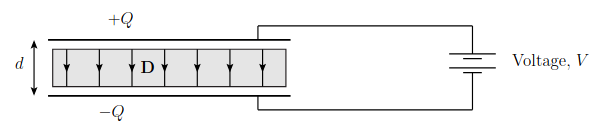
\includegraphics[width=0.5\textwidth]{dielecetric capacitor.png}
	\caption{The boundary between two dielectric materials. Each region has a distinct relative permitivity, denoted by $\varepsilon^{(1)}_r$ and $\varepsilon^{(2)}_r$.}
	\label{fig:dielectric capacitor}
\end{figure}
Consider a parallel plate capacitor with a dielectric, as in fig. \ref{fig:dielectric capacitor}. The surface charge of the plate is given by $\sigma_P \frac{Q}{A}$. By eq. \eqref{eq:d field}, we have,
\begin{equation}
	\oint \vb{D}\cdot{\dd{\vb{S}}} = D_z A = Q.
\end{equation}
We can then write that the $z$ component of the electric field is,
\begin{equation}
	E_z = \frac{Q}{(1 + \chi_E)\varepsilon_0 A}
\end{equation}
and the $z$ component of the polarisation field is,
\begin{equation}
	P = \frac{\chi_E Q}{(1 + \chi_E)A}.
\end{equation}
The potential difference between the plates is,
\begin{equation}
	\Delta \phi = E_z d = \frac{Qd}{(1 + \chi_E)\varepsilon_0A}
\end{equation}
so the capacitance is,
\begin{equation}
	\begin{split}
		C = \frac{Q}{\Delta \phi} & = (1 + \chi_E)\frac{\varepsilon_0A}{d}\\
		& = (1 + \chi_E)C_0
	\end{split} \label{eq:fhj}
\end{equation}
where $C_0$ is the capacitance in vacuum. Eq. \eqref{eq:fhj} holds at constant $Q$ with out a battery connected. From this, we can conclude that the electric field is lowered by $(1 + \chi_E) = \varepsilon_r$ due to the dieelectric. So, we can rewrite the electric displacement vector as,
\begin{equation}
	\boxed{\vb{D} = \varepsilon_r\varepsilon_0\vb{E}}. \label{eq:d form}
\end{equation}
\subsubsection{Energy in a capacitor}
We know trivially,
\begin{equation}
	u = \frac{1}{2}C \Delta \phi^2 =  \frac{\frac{1}{2}A\varepsilon_r\varepsilon_0\left(E_zd^2\right)}{d} = \frac{1}{2}AdD_zE_z
\end{equation}
in the $z$ direction for a parallel plate capacitor. However, generally,
\begin{equation}
	u = \frac{1}{2}\int \vb{D}\cdot\vb{V}\dd{V}.
\end{equation}
\subsection{Interfaces between Dielectrics}
\begin{figure}
	\centering
	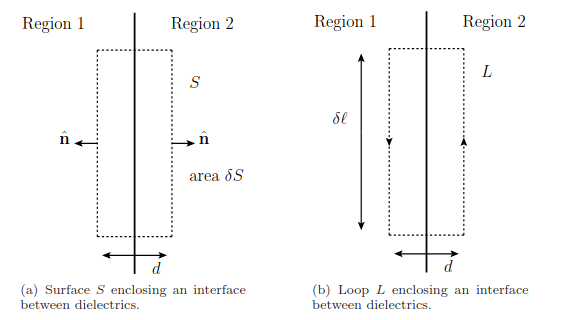
\includegraphics[width=0.75\textwidth]{interface.png}
	\caption{}
	\label{fig:interface}
\end{figure}
\subsubsection{Electric diplacement between two materials}
Consider fig. \ref{fig:interface} (a), where we have a gaussian surface $S$ enclosing the boundary between the two materials, with thickness $d$ and area $\delta S$. When we take $d \to 0$, let us assume no free charges at the boundary. We then have,
\begin{equation}
	\begin{split}
	\oint\vb{D}\cdot\dd{\vb{S}} & = 0 = -D_{\perp}^{(1)}\delta S + D_{\perp}^{(2)}\delta S \\
	& \implies D_{\perp}\text{ is continous at the boundary.}
	\end{split}
\end{equation}
\subsubsection{Electric field between two materials}
Let us now consider fig. \ref{fig:interface} (b). Let us consider a loop $L$ enclosing the boundary, with length $\dd{\ell}$ and width $d$. We assume no surface charges. Then, as $d \to 0$,
\begin{equation}
	\begin{split}
	\oint \vb{E} \cdot\dd{\vb*{\ell}} & = 0 = E_{\parallel}^{(1)}\delta \ell + E_{\parallel}^{(2)}\delta\ell \\
	& \implies E_{\parallel}\text{ is continuous across the boundary.}
	\end{split}
\end{equation}
\subsubsection{The general case}
\begin{figure}
	\centering
	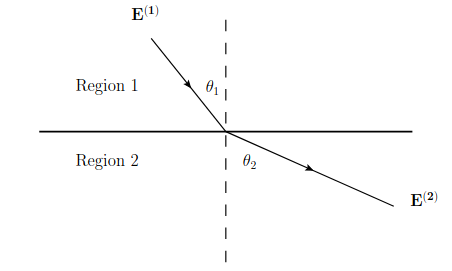
\includegraphics[width=0.75\textwidth]{interface1.png}
	\caption{}
	\label{fig:interface2}
\end{figure}
Let us consider fig. \ref{fig:interface2}. The electric field in the two regions is,
\begin{align}
	\vb{E}^{(1)} = E_1\begin{pmatrix}
		\sin\theta_1 \\ \cos\theta_1
	\end{pmatrix} && \vb{E}^{(2)} = E_2\begin{pmatrix}
	\sin\theta_2 \\ \cos\theta_2
	\end{pmatrix}
\end{align}
If $E_{\parallel}$ is continous,
\begin{equation}
	E_1\sin\theta_1 = E_2\sin\theta_2. \label{eq:239}
\end{equation}
If $D_{\perp}$ is continuous,
\begin{equation}
	D_1\cos\theta_1 = D_2\cos\theta_2. \label{eq:532}
\end{equation}
Dividing eq. \eqref{eq:532} by eq. \eqref{eq:239}, 
\begin{equation}
	\frac{D_1}{E_1}\cot\theta_1 = \frac{D_2}{E_2}\cot\theta_2
\end{equation}
and by eq. \eqref{eq:d form},
\begin{equation}
	\varepsilon_r^{(1)}\cot\theta_1 = \varepsilon_r^{(2)}\cot\theta_2.
\end{equation}
From these we can get key relations for dielectrics at boundaries,
\newtcolorbox{mybox}{width=0.4\textwidth,
	halign=justify,
	center,
	breakable,
	colback=white }
\begin{mybox}
	\begin{align}
		\frac{D_1}{D_2} & = \frac{\cos\theta_2}{\cos\theta_1} \\
		\frac{D_1}{D_2} & = \frac{\epsilon_1 \sin\theta_2}{\epsilon_2 \sin\theta_1} \\
		\frac{\epsilon_1}{\epsilon_2} & = \frac{\tan\theta_1}{\tan\theta_2}
	\end{align}
\end{mybox}
\section{Inductance and Relative Permeability}
Recall...\\\\
\begin{tcolorbox}
For a long solenoid of length $L$, current $I$, $n$ turns per unit length, and distance $r$ from the centre of the solenoid, the magnetic field is given by,
\begin{equation}
	B = \mu_0 nI.
\end{equation}
The flux through the solenoid is given by,
\begin{equation}
	\begin{split}
	\Phi_B = \int \vb{B}\cdot\dd{S} & = \pi r^2 n l B \\
	& = \mu_0 n^2 \pi r^2 l I.
	\end{split}
\end{equation}
By Faraday's law the EMF throuhg the coil is,
\begin{equation}
	\epsilon = -\pdv{\Phi_B}{t} = -\mu_0n^2\pi r^2 l \pdv{I}{t},
\end{equation}
and we define the inductance,
\begin{equation}
	\mathcal{L} = -\frac{\epsilon}{I} = \mu_0 n^2 \pi r^2 l
\end{equation}
measured in Henrys $\left[\text{H}\right]$.
\end{tcolorbox}
\noindent
The above is true in a vaccuum. Similarly as we did for electrostatics, we wish to formulate magnetostatics in materials. Let us begin by definiing some quantities.
\\\\
The relative permeability is given by,
\begin{equation}
	\mu_r = \frac{\mathcal{L}}{\mathcal{L}_{\text{vacuum}}}.
\end{equation}
Let us define the magnetic dipole moment,
\begin{equation}
	\vb{m} = IA\vu{n}.
\end{equation}
where the torque and potential are given by,
\begin{align}
	u_{\text{ext}} = -\vb{m}\cdot\vb{B}_{\text{ext}} && \vb*{\tau}_{\text{ext}} = \vb{m}\cross\vb{B}_{\text{ext}}.
\end{align}
We then define the \textit{magnetisation},
\begin{equation}
	\vb{M} = n\vb{m}.
\end{equation}
We then define the \textit{magnetic susceptibility} such that,
\begin{equation}
	\vb{M} = \frac{\chi_B}{\mu_0}\vb{B} \label{eq:magnetic sus}
\end{equation}
for a linear, isotropic response.
\\\\
We will be considering 3 different types of magnetisation, described in the sections below. Diamagnetism and paramagnetism occur in non-magnetic materials, while ferromagnetism occurs in magnetic materials.
\subsection{Diamagnetism}
This occurs for the case $\chi_B < 0$. Let us imagine an electron orbiting a nucleus, which will result in a current,
\begin{equation}
	I = \frac{ev}{2\pi r}.
\end{equation}
We want to obtain the magnetic moment,
\begin{equation}
	m = \frac{ev}{2\pi r}\pi r^2 = \frac{e}{2m_e}J
\end{equation}
where $J$ is the angular momentum such that $J = m_erv$. Current flows in the direction of positive charges, so,
\begin{equation}
	\vb{m} = - \frac{e}{2m_e}\vb{J}.
\end{equation}
From quantum mechanics, we understand that orbital angular momentum of the electron is qunatised such that,
\begin{equation}
	\left|\vb{J}\right| = \sqrt{\ell(\ell + 1)}\hbar
\end{equation}
so we have that the magnetic dipole moment is directly proportional to the \textit{Bohr magneton}, which encodes the spin of the electron, such that,
\begin{align}
	\mu_B \propto |\vb{m}| && \mu_B = \frac{e\hbar}{2m_e}.
\end{align}
For an ato with multiple electrons, we have 
\begin{equation}
	\vb{m}_{\text{tot}} = \sum_i m_i = -\frac{e}{2m_e}\sum_i\vb{J}_i.
\end{equation}
For Diagmetism, there is no intrinsic dipole moment, so we have that $\sum_i \vb{L}_i = 0$.
\\\\
Let us consider the force on $Z$ electrons where there is no applied magnetic field, 
\begin{equation}
	|\vb{F}| = mr\omega^2 = q|\vb{E}| \implies m_e \omega_0^2 r = \frac{Ze}{4\pi\varepsilon_0 r^2}
\end{equation} 
which can be rearranged to obtain the rotational frequency,
\begin{equation}
	\omega_0 = \sqrt{\frac{Ze^2}{4m_e\varepsilon_0 r^2}}.
\end{equation}
Let us suppose there is a small, instantaneous displacement in the external magnetic field $\delta \vb{B}_{\text{ext}}$. By the Lorentz force, we have,
\begin{equation}
	m_e \omega^2 r = \frac{Ze^2}{4\pi \varepsilon_0 r^2} + e\omega r \delta B_{\text{ext}},
\end{equation}
from which we can write the displacement in angular momentum,
\begin{equation}
	|\delta \vb{J}| = \frac{1}{2}er_0^2\delta B_{\text{ext}}.
\end{equation}
We should note that we are performing a classical approximation where we really require a quantum mechanical description of the perturbation of the system. Continuing, however, we can write the induced magnetic dipole moment is given by,
\begin{equation}
	\vb{m}_{\text{ind}} = -\frac{e\delta J}{2me} = -\frac{e^2r_0^2}{4m_e}\vb{B}_{\text{ext}}.
\end{equation}
For $Z$ electrons, averaging over all orientations of electron orbits, the induced magnetic dipole moment and the corresponding magnetisation is given by,
\begin{align}
	\boxed{\vb{m} = -\frac{e^2}{6m_e}Z\left<r^2\right>\vb{B}_{\text{ext}}} && \boxed{\vb{M} = -\frac{ne^2Z\left<r^2\right>}{6m_e}\vb{B}_{\text{ext}}}
\end{align}
which describes diamagnetism.
\subsection{Paramagnetism}
Paramagnetism occurs when $\sum_i\vb{L}_i \neq 0$, which results in an intrinsic dipole moment $\vb{m}_\text{int}$. We then have that the extrenal magnetic field creates an alignment,
\begin{equation}
	\vb{M} = \frac{nm_{\text{int}^2}}{3k_B T}\vb{B}_{\text{ext}}.
\end{equation}
\subsubsection{Magnetic Susceptibility}
We are then able to write the overall magnetic susceptibility due to effects of both paramagnetism and diamagnetism,
\begin{equation}
	\boxed{\chi_B = \mu_0n\left(\frac{m_{\text{int}^2}}{3k_BT} - \frac{Ze^2\left<r^2\right>}{6m_e}\right)}
\end{equation}
In paramagnetism, it was assumed that intrinsic dipoles did not interact. HOwever, in certain materials, this is not the case.
\section{Magnetostatics in a Magnets}
As in the electrostatic case, we will attempt to distinguish between bound and free currents. In a magnet, there are bound currents such that,
\begin{equation}
	\vb{J}_{\text{bound}} = \curl{\vb{M}}
\end{equation}
which correspond to internal, non-observed currents. We will further have surface currents for where charge carriers align at the surface to provide a net current,
\begin{equation}
	\vb{J}_{\text{surface}} = \vb{M} \cross \vu{n}
\end{equation}
where $\vu{n}$ is the normal to the surface. Let us recall equations of magnetostatics,
\begin{align*}
	\div{\vb{B}} = 0 && \curl{\vb{B}} = \mu_0 \vb{J}.
\end{align*}
Let us seperate the total current density $\vb{J}$ into bound and free components, beginning with Ampere's law,
\begin{equation}
	\begin{split}
		\curl{\vb{B}} & = \mu_0\left(\vb{J}_{\text{bound}} + \vb{J}_{\text{free}}\right) \\
		& = \mu_0\curl{\vb{M}} + \mu_0\vb{J}_{\text{free}}.
	\end{split}
\end{equation}
By trivial rearrangement, we can define the $\vb{H}$ field,
\begin{equation}
	\boxed{\vb{H} \equiv \frac{1}{\mu_0}\vb{B} - \vb{M}}
\end{equation}
with units $\left[\text{A m}^{-1}\right]$, such that,
\begin{equation}
	\boxed{\curl{\vb{H}} = \vb{J}_{\text{free}}}
\end{equation}
with integral form,
\begin{equation}
	\boxed{\oint\vb{H} \cdot \dd{\vb*{\ell}} = I_{\text{free}}}.
\end{equation}
\subsection{Properties of the $\vb{H}$ field}
By \eqref{eq:magnetic sus}, we have,
\begin{equation}
	\vb{H}= \frac{1 - \chi_E}{\mu_0}\vb{B}. \label{eq:fdsh}
\end{equation}
The magnetic energy is given by,
\begin{equation}
	u = \frac{1}{2}\int\vb{B}\cdot\vb{H} \dd{V}.
\end{equation}
For a solenoid of length $\ell$,
\begin{equation}
	\begin{split}
		&\int\vb{H} \cdot\dd{\vb*{\ell}} = H\ell = N\ell I \\
		\implies & H = NI
	\end{split}
\end{equation}
By eq. \eqref{eq:fdsh}, we get the EMF,
\begin{equation}
	\varepsilon = - \frac{\mu_0 N^2\pi r^2 \ell}{1 - \chi_B}\dv{I}{t}.
\end{equation}
The inductance is then given by,
\begin{equation}
	\mathcal{L} = \frac{\varepsilon}{I} = \frac{\mathcal{L}_{\text{vac}}}{1 - \chi_B}.
\end{equation}
We can then redefine the relative permeability as,
\begin{equation}
	\mu_r = \frac{1}{1 - \chi_B}
\end{equation}
and thus, writing the magnetic field in terms of $\vb{H}$,
\begin{equation}
	\boxed{\vb{B} = \mu_r\mu_0 \vb{H}}. \label{eq:H}
\end{equation}
\subsection{Interfaces between Magnetic Materials}
By similar reasoning as the electrostatic case, we find that at the boundary between two different magnetic materials of relative permeabilities $\mu_r^{(1)}$ and $\mu_r^{(2)}$ we have,
\begin{align}
	\oint \vb{H}\cdot\dd{\vb*{\ell}} = 0 \implies \vb{H}_{\parallel} \text{ is continuous at the boundary} \\
	\oint \vb{B}\cdot\dd{\vb{A}} = 0 \implies \vb{B}_{\perp} \text{ is continuous at the boundary}
\end{align}
\subsection{Potential formulation}
If $\vb{M}$ is constant, there are no bound currents, and only surface currents are present. Given this, we can say that,
\begin{equation}
	\curl{\vb{H}} = 0
\end{equation}
which allows s to define an \textit{effective magnetic charge},
\begin{equation}
	\div{\vb{H}} = - \div{\vb{M}} = \rho_{M}.
\end{equation}
This allows us to formulate an equation for $\vb{H}$ in terms of a potential,
\begin{equation}
	\vb{H} = - \grad \psi.
\end{equation}
From this, we are able to write a poisson equation for the magnetic potential $\psi$,
\begin{equation}
	\boxed{\grad^2\psi = -\psi_m = \div{\vb{M}}} 
\end{equation}
which gives way to a solution,
\begin{equation}
	\boxed{\psi(r) = - \frac{1}{4\pi r}\int \dd{V}' \frac{\div{\vb{M}(\vb{r}')}}{|\vb{r} - \vb{r}'}}
\end{equation}

\section{Ferromagnetism}
In paramagnetism, we assumed that intrinsic dipoles did not interact. However, in ferromagnetic magterials this is not the case. Within materials, there are ferromagnetic domains, which are areas of material which have the same dipole alignment. Furthermore, eq. \eqref{eq:magnetic sus} and eq. \eqref{eq:H} no longer hold. Instead we have relations,
\begin{align}
	\vb{M} \equiv \vb{M}(\vb{B}) && \mu_r = \frac{1}{\mu_0}\pdv{B}{H}.
\end{align} 
If we have 2 magnetic moments $\vb{m}_1$ and $\vb{m}_2$, the energy associated with their alignments are,
\begin{equation}
	\Delta u_{12} = - \vb{m}_1\cdot \vb{m}_2.
\end{equation}
To reduce energy, we must align the moments such that,
\begin{equation}
	\vb{m}_1 \propto \vb{m}_2.
\end{equation}
\subsection{Formation of Domains}
\begin{figure}
	\centering
	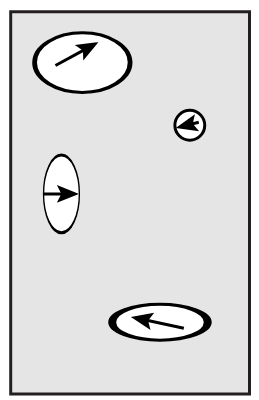
\includegraphics[width=0.1\textwidth]{T=T_c - Epsilon.png}
	\caption{}
	\label{fig:t - e}
\end{figure}
\begin{figure}
	\centering
	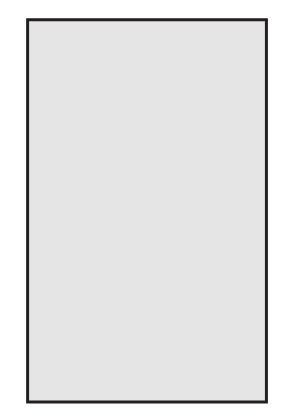
\includegraphics[width=0.1\textwidth]{T_T_C.png}
	\caption{}
	\label{fig:t=tc}
\end{figure}
\begin{figure}
	\centering
	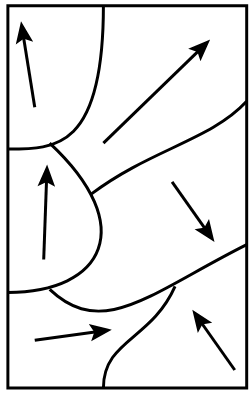
\includegraphics[width=0.1\textwidth]{T__T_C.png}
	\caption{}
	\label{fig: t < tc}
\end{figure}
Domains form at different temperatures. We will define the \textit{Curie temperature} $T_C$ at which domains no longer exist. Below we describe the effects on ferromagnets at different temperatures,
\begin{enumerate}
	\item $T >> T_C$, as in fig. \ref{fig:t=tc}. The interactions between magnetic dipoles are weak due to thermal fluctuations dominating. The material presents only paramagnetic effects.
	\item $T = \lim_{\epsilon \to 0}(T_C - \epsilon)$, as in fig. \ref{fig:t - e}. Interactions between dipoles begin to have effects, and bubbles of magnetic dipoles form. This process is known as "bubble nucleation".
	\item $T << T_C$, as in fig. \ref{fig: t < tc}. Domains grow and the whole substance is partitioned into a domain.
\end{enumerate}
\subsection{Ideal ferromagnets}
In an ideal ferromagnet, $M$ is constant within the material. This often occurs at or near $T = 0$K. This means that there is a single magnetic domain in the material. For a material with atomic weight $A$, its number density for magnetic dipoles is,
\begin{equation}
	n = \frac{N_AR}{A}.
\end{equation}
Its approximate magnetisation is going to be defined by the Bohr magneton, such that $n\mu_B$. The magnitude of its magnetisation is going to be,
\begin{equation}
	|\vb{M}| \approx S n \mu_B
\end{equation}
where $S$ is a random small integer. Therefore, our magnetic field has an approximate magnitude of,
\begin{equation}
	|\vb{B}| \approx \mu_0 |\vb{M}|
\end{equation}
which results in a magnitude of a few teslas, which is a very strong magnetic field.
\subsection{Potential formulation for an ideal ferromagnet}
We can rewrite the solution to Poisson's equation for a ferromagnet as,
\begin{equation}
	\boxed{\frac{1}{4\pi}\div{\int{\dd{V}'\frac{\vb{M}(\vb{r}')}{|\vb{r}- \vb{r}'|}}}}
\end{equation}
\subsubsection{Example: Uniformly Magnetised Sphere}
Consider a uniformly magnetised sphere of radius $a$ at a temperature $T=0$. We assume it has a uniform magnetisation,
\begin{equation}
	\vb{M} = \begin{cases}
		M_0\vu{z} & r < a \\
		0 & r > a
	\end{cases}.
\end{equation}
Going forth with this, we find that the magnetic scalar potential is,
\begin{equation}
	\psi = \frac{1}{3}M_0\begin{cases}
		z & r < a \\
		\frac{1}{r^2}a^3\cos\theta & r>a
	\end{cases}
\end{equation}
which can give us further insight into how the $B$ and $H$ fields behave. We find that outside the magnetised sphere, it behaves as a dipole, with $\vb{B} = \mu_0\vb{H}$. Whereas inside the sphere, we find,
\begin{align}
	\vb{H} = - \grad\psi = -\frac{1}{3}M_0\vu{z} \\
	\vb{B} = \mu_0(\vb{H} + \vb{M}) = \frac{2}{3}\mu_0M_0\vu{z}
\end{align}
\begin{figure}
	\centering
	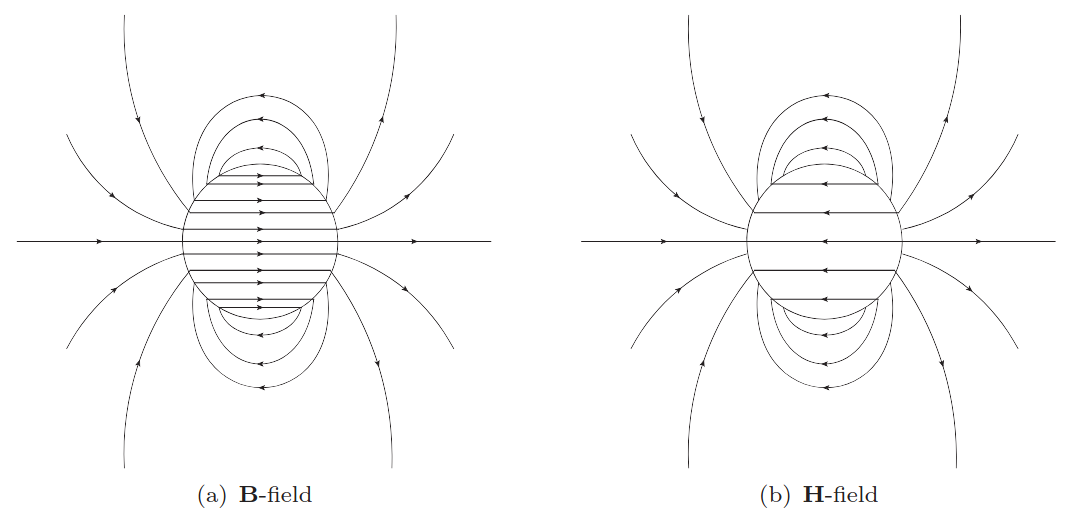
\includegraphics[width=0.7\textwidth]{B-H.png}
	\caption{}
	\label{fig:bh}
\end{figure}
The key differences in the behaviour of the two fields is summarised below, and visualised in figure \ref{fig:bh},
\begin{itemize}
	\item As $M\uparrow$, $H\downarrow$.
	\item $\vb{B}$ and $\vb{H}$ are anti-parallel.
	\item $\vb{H}$ is lower than $\vb{B}$ inside the ferromagnet, and points in the opposite direction.
	\item For $T>0$ the relationship between $\vb{B}$ and $\vb{H}$ becomes far more complicated.
\end{itemize}
\subsection{Electromagnets and Hysteresis}
\begin{figure}
	\centering
	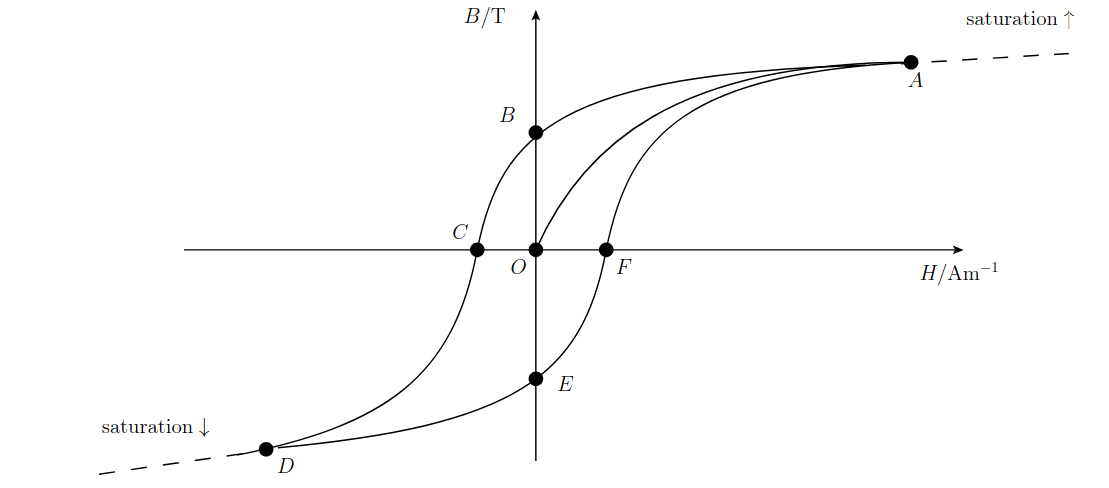
\includegraphics[width=0.7\textwidth]{B-H graph.png}
	\caption{}
	\label{fig:bhgraph}
\end{figure}
If we consider a wire wrapped around a ferromagnet, the wire carries a current $I$. Since $\vb{H} = \vb{H}(I)$, we can control th emagnetic intensity vector $\vb{H}$. AS currernt is applied, the domains begin to flip and $\vb{H}$ will increase alongside $\vb{B}$. We have that $\vb{M} \propto \vb{B}$. The magnetisation will eventually reach a maximum (point $A$ on figure \ref{fig:bhgraph}) $\vb{M} = \vb{M}_{\text{Max}}$. All domains are aligned, and can only slowly increase $\vb{H}$.
\\\\
If we decide to then lower the current, we find that the magnetisation is non-zero at $\vb{H} = 0$, i.e., some domains have been permanently aligned. If we then increase current but in the opposite direction, all the domains flip and cancel out the magnetic field. At point $C$ in figure \ref{fig:bhgraph}, we have $\vb{H} = \vb{H}_C$ which is known as the coercive field. 
\\\\
The work done is given by the area under the hysterisis curve in figure \ref{fig:bhgraph}, given by,
\begin{equation}
	\int U = -V \oint \vb{H} \cdot{\dd{\vb{B}}}.
\end{equation} 
\chapter{Electromagnetic Waves} 
\section{Solutions to the Wave Equation in 1D}
The general wave equation is given by
\begin{equation}
	\frac{1}{v^2}\pdv[2]{\phi}{t} - \pdv[2]{\phi}{x} = 0. \label{eq:11}
\end{equation}
The most general solutoin is given by,
\begin{equation}
	\phi(x,t) = f(x-vt) + g(x + vt).
\end{equation}
We can trial a plane wave ansatz,
\begin{equation}
	\phi(x,t) = Ae^{i(kx-\omega t)} + Be^{i(kx +\omega t)}. \label{eq:22}
\end{equation}
If we substitute eq. \eqref{eq:22} into \eqref{eq:11}, we obtain the dispersion relation,
\begin{equation}
	\omega = vk.
\end{equation}
The wave's phase is given by,
\begin{equation}
	\psi = kx - \omega t
\end{equation}
and hence parts of the wave with the same phase is given by,
\begin{equation}
	\psi = \frac{2\pi}{n}
\end{equation}
thus we have,
\begin{equation}
	kx - \omega t = 2\pi n. 
\end{equation}
Let us recall that phase velocity and group velocity are given by,
\begin{align}
	v_p = \frac{\omega}{k} && v_g = \pdv{\omega}{k}
\end{align}
respectively. We require $\phi$ to be a real scalar field, so the physical part of the solution,
\begin{equation}
	\Re{\phi} = |A|\cos(kx - \omega t)
\end{equation}
given the argument of $A$ is 0. 
\subsection{Wave Equation in 3D}
The wave equation is given by,
\begin{equation}
	\frac{1}{v^2} \pdv[2]{\phi}{t} - \laplacian{\phi} = 0. \label{eq:33}
\end{equation}
Whose solution is given by,
\begin{equation}
	\phi = Ae^{i(\vb{k}\cdot\vb{r} - \omega t)} + B e^{i(\vb{k}\cdot\vb{r} + \omega t)}
\end{equation}
where $\vb{r}$ is an arbitrary position vector. The direction of propogation of the wave is given by $\vu{k}$, where,
\begin{equation}
	\vb{k} = \frac{2\pi}{\lambda}\vu{k}.
\end{equation}
If $B$ = 0, we have,
\begin{equation}
	\pdv{\phi}{x} = ik_x Ae^{i(\vb{k}\cdot{\vb{r}} - \omega t)} = ikx \phi \label{eq:44}
\end{equation}
Furthermore,
\begin{align}
	\grad \phi = i\vb{k}\phi \label{eq:55}\\
	\laplacian \phi = |\vb{k}|^2 \phi \label{eq:66}\\
	\pdv[2]{\phi}{t} = - \omega^2 \phi \label{eq:77}
\end{align}
If we substitute eq. \eqref{eq:66} and eq. \eqref{eq:77} into \eqref{eq:33}, we obtain the dispersion relation,
\begin{equation}
	\omega = v|\vb{k}|,
\end{equation}
and,
\begin{equation}
	\vb{k}\cdot\vb{r} - \omega t = 2\pi n.
\end{equation}
\section{Maxwell's Equations in Free Space and the Electric Wave Equation}
The conditions for free space are $\rho =0$ and $\vb{j} = 0$, which gives us,
\begin{align}
	\div{\vb{E}} = 0 && \div{\vb{B}} = 0 \\
	\Dot{\vb{B}} = -\curl{\vb{E}} && \Dot{\vb{E}} = c^2 \curl{\vb{B}} \label{eq:ab}.
\end{align}
Let us consider the time derivatives of eqs. \eqref{eq:ab},
\begin{equation}
	\begin{split}
		\Ddot{\vb{E}} = c^2 \curl{\Dot{\vb{B}}} & = -\left(\curl{(\curl{\vb{E}})}\right) 
		 = -c^2\left(\grad(\cancelto{0}{\div{\vb{E}}} - \laplacian{\vb{E}})\right)
	\end{split}
\end{equation}
for which we obtain our final relation,
\begin{equation}
	\boxed{\frac{1}{c^2}\Ddot{\vb{E}} - \laplacian \vb{E} = 0} \label{eq:88}
\end{equation}
which is a wave equation in 3D. We can follow a similar procedure for the magnetic field,
\begin{equation}
	\boxed{\frac{1}{c^2}\Ddot{\vb{B}} - \laplacian\vb{B} = 0}. \label{eq:99}
\end{equation}
Eqs. \eqref{eq:88} and \eqref{eq:99} imply that the electric and magnetic fields are both plane waves moving at speed $c$. We can use the plane wave ansatz,
\begin{align}
	\vb{E}= \vb{E}_0 e^{i(\vb{k}\cdot\vb{r} - \omega t)} && \vb{B} = \vb{B}_0e^{i(\vb{k}\cdot\vb{r} - \omega t)}
\end{align}
where $\vb{E}_0$ and $\vb{B}_0$ are the polarisation vectors. 
\subsection{Relationship between $\vb{E}$ and $\vb{B}$}
Let us consider a general monochromatic wave,
\begin{align}
	\div{\vb{E}} = i\vb{k}\cdot\vb{E} && \curl{\vb{E}} = i\vb{k}\cross \vb{E}.
\end{align}
By Gauss's law,
\begin{equation}
	\vb{k}\cdot\vb{E} = 0
\end{equation}
$\implies$ $\vb{k}$ and $\vb{E}$ are orthogonal, i.e., the direction of propogation is orthogonal to the electric field. Now, considering the magnetic field,
\begin{equation}
	-\Dot{\vb{B}} = \curl{\vb{E}} = i\vb{k}\cross\vb{E}_0e^{i(\vb{k}\cdot\vb{r} - \omega t)}
\end{equation}
which, integrated, gives,
\begin{equation}
	\vb{B} = \vb{k}\cross \frac{\vb{E}_0}{\omega}e^{i(\vb{k}\cdot{\vb{r}} - \omega t)}
\end{equation}
$\implies$ $\vb{B}$ is orthogonal to $\vb{E}$.
\appendix 
\chapter{Proofs}
\section{Loop integral over perfect differential}
\begin{proof}
	\begin{equation}
		\oint_L \dd{\vb*{\ell}} \cdot \grad f \underbrace{=}_{\text{Stoke's theorem}} \int_S \dd{\vb{S}} \cdot\left(\underbrace{\curl{\grad f}}_0\right) = 0
	\end{equation}
\end{proof}
\chapter{Examples}
\section{Coloumb's law for two, straight, parallel wires}
The force on an infinitesimal line element is,
\begin{equation}
	\vb{F}_{12} = I_1\dd{\vb*{\ell}}\cross\vb{B}_2\left(\vb{r}_1\right).
\end{equation}
The magnetic field due $\vb{B}_2$ due to wire 2 is given by,
\begin{equation}
	\vb{B}_2\left(\vb{r}\right) = \frac{\mu_0 I_2}{2\pi\left|\vb{r} - \vb{r}_2\right|}\vu*{\theta},
\end{equation}
thus,
\begin{equation}
	\dd{\vb{F}_{12}} = \frac{\mu_0 I_1I_2}{2\pi d}\dd{\ell}\vu{z}\cross\vu*{\theta},
\end{equation}
where $\vu{z}\cross\vu*{\theta} = - \vu{r}$, thus,
\begin{equation}
	\dv{F_{12}}{\ell} = \pm \frac{\mu_0 I_1I_2}{2\pi d}
\end{equation}
where we have an attractive force if both currents are travelling in the same direction.
\section{Coloumb's law for two parallel current carrying wires}
If we define current $I\dd{\vb*{\ell}} = q\vb{v}$, then the magnetic force is given by,
\begin{equation}
	 I \dd{\vb*{\ell}} = q\vb{v}.
\end{equation}
We have that the force on wire 1 due to wire 2 is,
\begin{equation}
	\begin{split}
		\vb{F}_{12} &= \oint_{L_1} I_1\dd{\vb*{\ell}_1} \cross \vb{B}_2(\vb{r}_1) \\
		& = \frac{\mu_0I_1I_2}{4\pi}\oint_{L_1}\dd{\vb*{\ell}_1}\cross\oint_{L_2}\dd{\vb*{\ell}_1} \cross \frac{\left(\vb{r}_1 - \vb{r}_2\right)}{\left|\vb{r}_1 - \vb{r}_2\right|^3} \\
		& = -\frac{\mu_0I_1I_2}{4\pi}\oint_{L_1}\oint_{L_2} \dd{\vb*{\ell}}_1\cdot\dd{\vb*{\ell}_2} \left(\frac{\left(\vb{r}_1 - \vb{r}_2\right)}{\left|\vb{r}_1 - \vb{r}_2\right|^3}\right)
	\end{split}
\end{equation}
We were able to rewrite the integral using the vector identity,
\begin{equation}
	\vb{v}_1 \cross \left(\vb{v}_2 \cross \vb{v}_3\right) = -(\vb{v}_1 \cdot \vb{v}_2)\vb{v}_3 + \vb{v}_2\left(\vb{v}_1 \cdot \vb{v}_3\right) \label{eq:id}
\end{equation}
and the second term in eq. \eqref{eq:id} in our case goes to 0 as we are performing a loop integral over a perfect differential.
\chapter{Interpretation of the Laplacian}
The laplacian of a scalar field $\phi$ is defined in cartesian coordinates,
\begin{equation}
	\laplacian{\phi} = \pdv{x_i}\pdv{x_i} \phi
\end{equation}
where we use the Einstein summation convention. Let us suppose a box with side length $a$. The average value of some $\phi$ in this box is,
\begin{equation}
	\bar{\phi} = \frac{1}{a^3}{\int\int\int}_V \phi \dd{x_1}\dd{x_2}\dd{x_3}. \label{eq:avg}
\end{equation}
If we consider the Taylor expansion about a point $\phi_0$ in the three coordinates, 
\begin{equation}
	\phi(x_i) = \phi_0 + \left(\pdv{x_i}\phi\right)_0x_i + \frac{1}{2}\left(\pdv{x_i}\pdv{x_j}\phi\right)_0x_ix_j + \cdots
\end{equation}
which can be substitued into eq. \eqref{eq:avg} and readily integrated to obtain,
\begin{equation}
	\bar{\phi} \cong \phi_0 + \frac{a^2}{24}\left(\pdv{x_i}\pdv{x_i}\phi\right)_0
\end{equation}
which rearranges to,
\begin{equation}
	\boxed{(\laplacian{\phi})_0 \cong \frac{24}{a^2}(\bar{\phi} - \phi_a)}.
\end{equation}
Thus, we can think of the laplacian at a point to be the measure of its difference with the average value of the field in the infinitesimal neighbourhood of that point. If we think about Poisson's equation ($\laplacian{\phi} = \rho$), from the intuition we developed, we see that Poisson's equation is saying that the difference from the average value about a point is proportional to the charge density. This makes sense, as at points of high charge density, the electric scalar field, and therefore the electric field lines, are going to be stronger, so the change of the scalar field at that point compared with the average field in the nieghbourhood will be higher as the field changes more.
\end{document}
